\documentclass[conference]{IEEEtran}
\usepackage{amsmath,amsfonts,amssymb}
\usepackage{graphicx}
\usepackage{color}
%\usepackage{url}

\begin{document}
\title{CS8803-O03 Reinforcement learning\\Project 2 report}

\author{\IEEEauthorblockN{Rohan D. Kekatpure}
\IEEEauthorblockA{Email: rdk@gatech.edu}}
% make the title area
\maketitle

% As a general rule, do not put math, special symbols or citations
% in the abstract
%\begin{abstract}
%\end{abstract}

\IEEEpeerreviewmaketitle
\section{Introduction}
The aim of this project is to train a reinforcement learning (RL) agent in a discrete-action continuous-state-space environment. The chosen agent is the lunar lander in the Box-2D environment. This project brings together many aspects of the course together and is a miniature version of latest advances in the field of RL. As such, despite the pain and nearly 100+ hours spent on this project, it has forced synthesis of the class material.
%%
\section{Quick theory tour}
The model-tree reinforcement learning (control) problem can be condensed into three equations:
\begin{align}
Q(s, a) &=f(s, a; w) \label{eq:fa} \\
\Delta w_t &= \alpha\left[r_{t+1} + \gamma \max_{a'}Q(s, a') - Q(s_t, a_t)\right] \label{eq:update} \\
a_{t+1} &= \arg\max_{a'} Q(s_{t+1}, a') \nonumber \\
& = \arg\max_{a'} f(s_{t+1}, a'; w_t)\label{eq:action},
\end{align}
where $Q(s, a)$ is the action-value function specifying the value of taking an action $a$ in state $s$. For large and/or continuous state spaces, the $Q$ function needs to be approximated. This approximation is expressed through the parameterized generalization function $f$. The {\bf optimal} next action is the one that yields largest $Q$ function value when evaluated with current parameters. Whether this action is {\bf chosen} or not depends on the exploit-explore strategy for the problem. The formulation also has a number of hyperparameters: the learning rate $\alpha$, the discount factor $\gamma$ and the exploration probability $\epsilon$. 

Note that there are alternative formulations of the problem. Particularly, the RL part can include more number of discounted states (e.g. TD(1) or Sarsa). The function approximation can be non-parameterized (nearest neighbors or table-lookup). But Eqs.~\eqref{eq:fa}--\eqref{eq:action} specify the mathematical formulation of the implementation presented in this report.   
%%
\section{Implementation methodology}
\subsection{Overview}
Our implementation for this project is a simplified version of the methodology presented in the DQN paper\cite{dqn}. While the RL part of the overall algorithm is identical to Algorithm 1 in the paper, our function approximation technique differs in from the DQN implementation in two important ways: (1) we use a simple, fully connected feed-forward neural network for function approximation (as opposed to convolutional net (CNN) in the DQN paper) and (2) our ``state'' is a combination of the 8-component vector provided by the environment and the {\bf one-hot-encoded} action vector. 

For $Q$ function generalization, we use a simple feed-forward neural network (motivation in \S~\ref{sec:expts1}) with two hidden layers of 50 nodes each and rectified activation. Our output layer is a single neuron without any activation. As a result of fusing the raw state with (encoded) action vector, our implementation needs to do 4 passes for the ``prediction'' part. The optimal action is the one that maximizes the output value.
%%
\subsection{Software dependencies}
Our solution is implemented within standard Python ecosystem; the only external dependencies are numpy and scikit-learn. In particular, we {\bf don't} use high-performance neural network learning frameworks such as Theano or Tensorflow, or their wrappers like Keras. 
%%
\section{Experiments}
\subsection{Choice of learner (``do we really need a neural net?'')}\label{sec:expts1}
RL success stories (TD-Gammon, Atari, Go) leave little doubt about the efficacy of neural nets as the function approximators. Yet, it is not obvious (at least to this author) why other supervised algorithms would not be able to outperform neural nets. To test the strength of other supervised algorithms on RL tasks, we experimented with linear, support-vector and decision tree learners (regressors). Table~\ref{tab:learners} summarizes the maximum average reward per 100 episodes that these learners were able to achieve. 
%%
\begin{table}[bpht]
\begin{center}
\begin{tabular}{|l|c|l|}
\hline
Learner & Max avg. reward & sklearn params \\ \hline 
Linear regression & $<-200$ & -\\
Support vector & $<-170$ & $C=0.01, \epsilon=0.2$ \\
Regression tree &$<-115$ & tree depth $\leq 15$ \\
Neural net & $> +55 $ & layers = $(50, 50), \alpha =10^{-3} $ \\ \hline
\end{tabular}
\end{center}
\caption{Maximum 100-episode average reward achieved by different learners on $Q$ learning. \label{tab:learners}}
\end{table}
%%

Our empirical evidence, though not exhaustive, hints to superiority of neural nets over other learning algorithms for $Q$ function generalization. One reason might be the non-linearity coupled with extreme non-convexity in the $Q$ function landscape. As a result, linear regression may have insufficient flexibility (i.e. high bias) to approximate the $Q$ function. In theory regression trees can approximate nonlinear and non-convex functions. Yet, in practice it may be difficult to search the hypothesis space efficiently in decision-tree representation. In addition, the hidden layers in neural nets have been interpreted to be representations of latent information in raw features (e.g. ``face-like'' or ``nose-like'' etc). This made it clear that we needed the expressive power of a neural net for $Q$-function approximation for this task.
%%
\subsection{Replay memory}
After failures with batch learning using a single episode, we settled on training in every step of every episode using uniform random sampling of the total experience (termed ``experience replay'' in the DQN paper). We noticed that training with states from a single episode makes the weights diverge. For our agent we fixed replay memory at 50000 and the batch size at 32.
%%
\subsection{Neural net parameters}\label{sec:nnparams}
\subsubsection{Hidden layers and batch size}
One drawback of neural network is the requirement for fine tuning of a number of hyper parameters. We ran a small number of experiments to get a general idea of the number of {\bf layers}, number of {\bf nodes per layer}, number of {\bf epochs} and the {\bf batch size}. It is computationally a difficult task to perform extensive parameter sweeps, so the choice of experiments is somewhat arbitrary. 

The fixed parameters for our neural net were warm start set to {\tt True} (i.e. use a momentum term), and ``adam'' as the SGD solver. As seen in Table~\ref{tab:nnarch}, the number of neural net training epochs per episode or larger number of hidden nodes don't necessarily lead to better fits. Reducing the epochs and hidden nodes does lead to significant speedup at the cost of a slight drop in max reward. As a result, out final neural net implementation used {\bf two} hidden layers with {\bf 50 nodes} each and a {\bf 32 sample} batch size.
%%
\begin{table}[bpht]
\begin{center}
\begin{tabular}{|c|c|c|c|c|c|c|}
\hline
layers & epochs & solver & iters & batch & speed & max rew\\ \hline 
(50, 50) & 50 & ``adam'' & 1000 & 128 & slow & +124 \\
(100, 100) & 50 & ``adam'' & 1000 & 256 & slow & +85 \\
(50, 50) & 20 & ``adam'' & 700 & 32 & ok & +132 \\
(50, 50) & 2 & ``adam'' & 700 & 32 & fast & +90 \\ \hline
\end{tabular}
\end{center}
\caption{Maximum 100-episode average reward achieved by different neural net architectures. \label{tab:nnarch}}
\end{table}
%
\subsubsection {Number of training epochs}
We train our neural net at each step of every episode. Allowing the neural net training to run for the default number of  epochs (200 in sklearn's {\tt MLPRegressor}) not only increases the training period, but also {\bf overfits} to the given batch. To speed up training and to avoid overfitting, we fixed number of training epochs per episode to 2. Figure~\ref{fig:lr}(a) demonstrates that a wrong choice of the training epochs can lead to under-training and unoptimized agents.
%%
\begin{figure}[tbp]
    \centering
    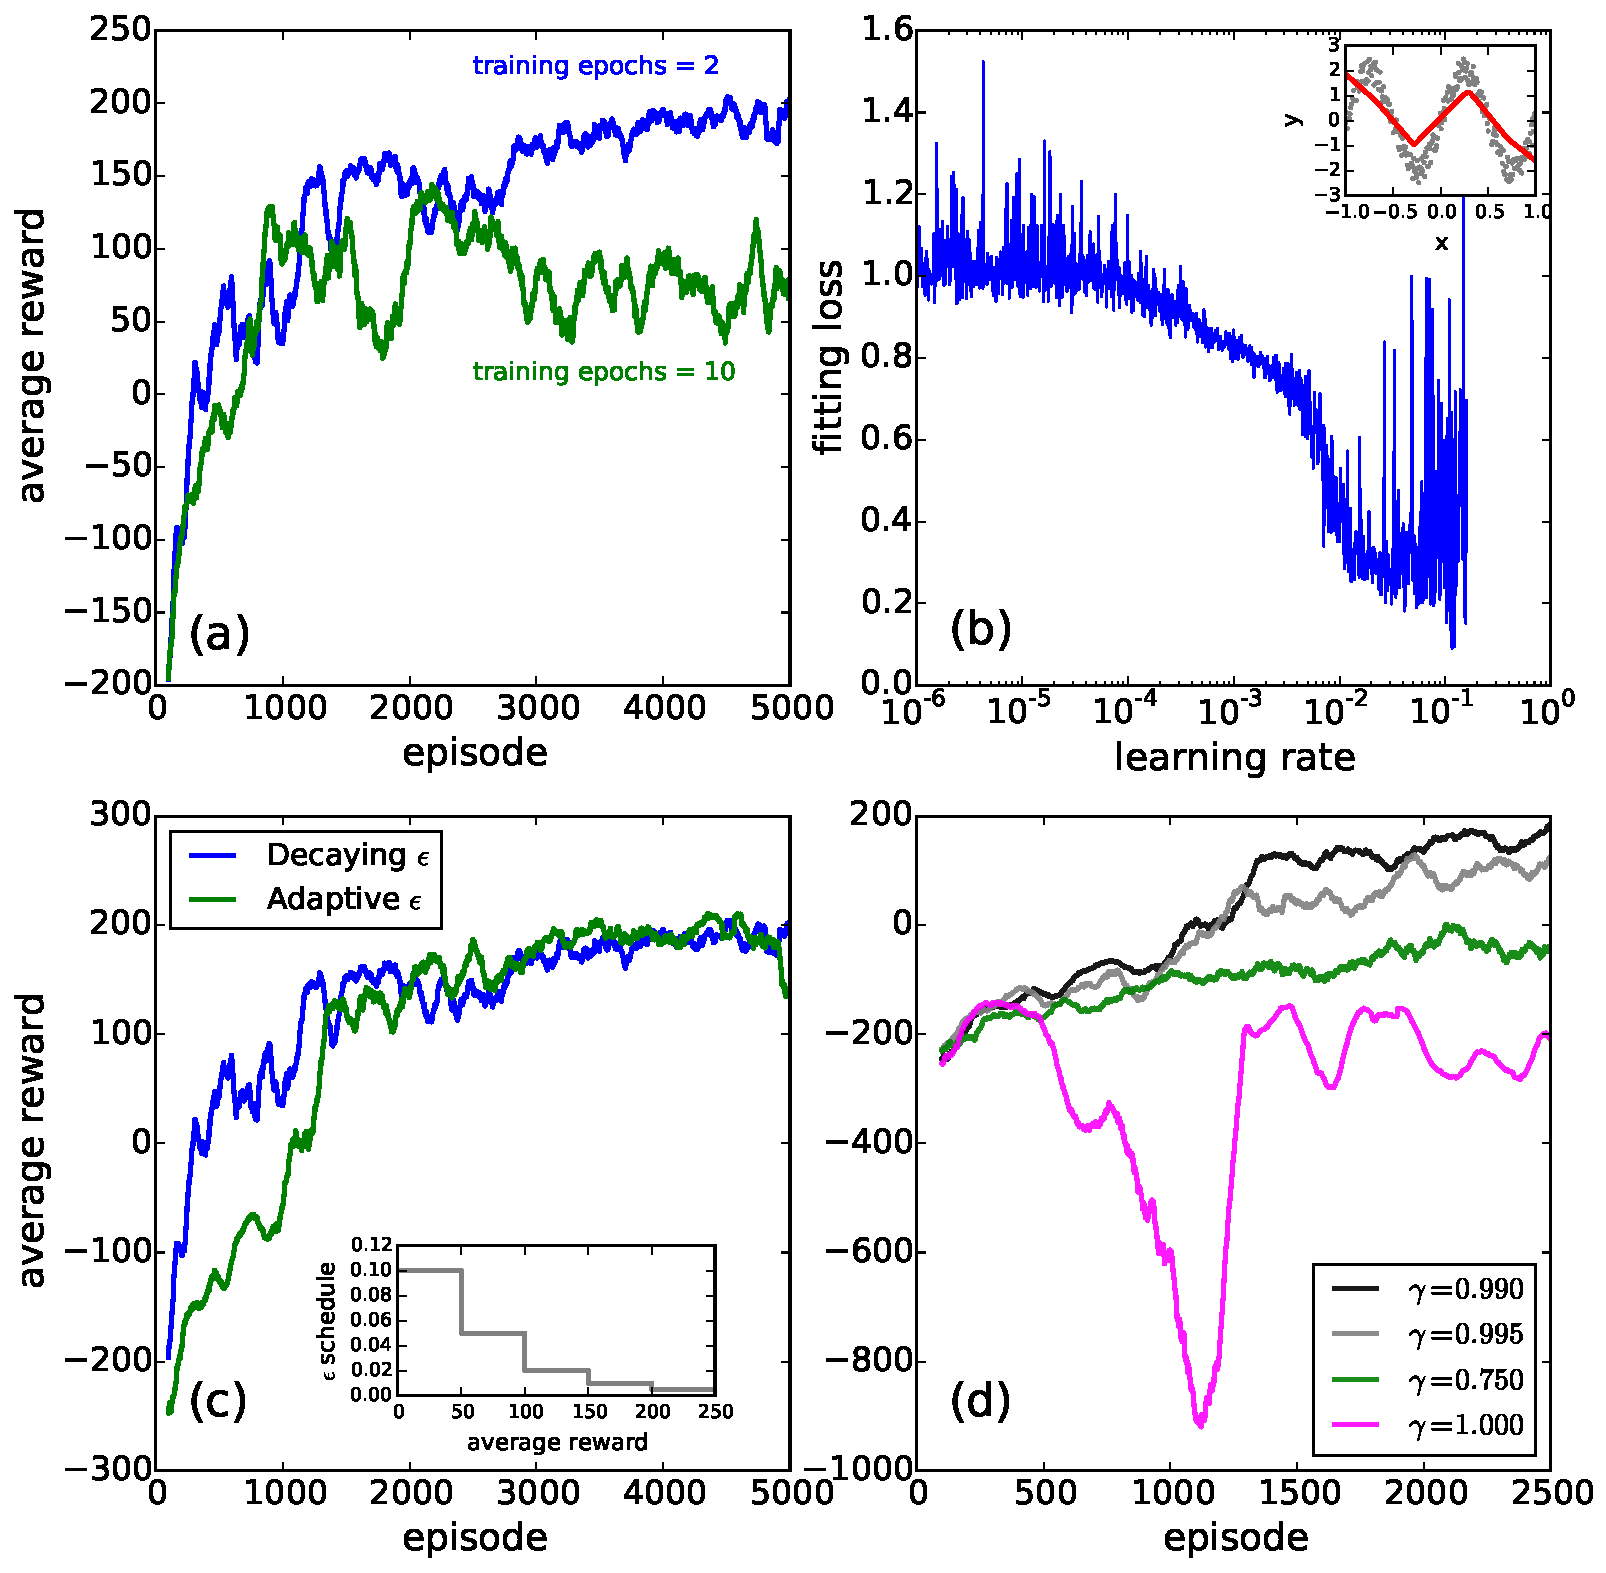
\includegraphics[width=0.5\textwidth]{./figures/fig0.pdf}
    \caption{Experiments on hyperparameter tuning. (a) Training effectiveness (100-episode average reward) vs episodes for two different epochs per episode. Optimal epochs per episode $\simeq 2$. (b) Learning rate ($\alpha$) vs fit quality measured using a 2-period sine wave(inset) fitted using our neural net regressor. Optimal learning rate $\simeq \alpha=10^{-4}$. (c) 100-episode average reward vs episodes for two different exploration strategies $\epsilon$. The {\color{blue} blue} curve is fixed geometric decay and {\color{green} green} curve is adaptive decay using the schedule shown in the inset. (d) 100-episode average reward for four discount factor $\gamma$ values shown in the legend. Optimal $\gamma = 0.990$\label{fig:lr}}
\end{figure}
%%
\subsubsection{Learning rate}
We estimated the optimal range of the learning rate $\alpha$ by fitting a 2 periods of a sine wave (Fig.~\ref{fig:lr}(b) inset) using the neural net fixed using the parameters defined in \S\ref{sec:nnparams}. The sine wave was selected as a proxy for a non-convex, nonlinear function. The learning rate vs the fit quality is plotted in Fig.~\ref{fig:lr}. It is clear that $\alpha>0.01$ can lead to unstable behavior even for this simple one-dimensional learning task. To keep the learning behavior stable we conservatively set our learning rate at a {\bf fixed } value of $\alpha = 10^{-4}$. This value offered a fast monotonic convergence.
%%
\subsection{Exploit-explore strategy}
The explore-exploit strategy is captured by the decay schedule for the $\epsilon$ parameter. We tried two different strategies, whose results are shown in Fig.~\ref{fig:lr}(c). The first experiment, shown in blue is standard time-dependent {\bf decay} in which we exponentially decay the initial $\epsilon$ until it reaches a minimum value:  $\epsilon_t \sim \max(\epsilon_{\text{min}}, \epsilon_0^t)$. The second strategy is {\bf adaptive} to the average reward; the exploration probability reduces near and optimum and jumps back up if the agent moves away from the optimum. This reward-adaptive schedule is shown in the inset to Fig.~\ref{fig:lr}(c). There is a slight difference between the initial learning speed, but the agent converge to similar terminal states. As a result we chose time-dependent $\epsilon$ decay schedule with $\epsilon_0=0.999$ and $\epsilon_{\text{min}}=0.01$.
%%
\subsection{Discount rate}
Typical episode length for the lunar lander is between 100 and 500--i.e. practically finite horizon. Our initial intuition therefore was that the discount rate would have little effect on the learning. Our experiments proved this intuition {\bf wrong}. As seen in Fig.~\ref{fig:lr}(d) the discount rate $\gamma$ hugely affects the rate of learning as well as the converged value. Our best performance was obtained at $\gamma = 0.990$. The performance deteriorated slightly for $\gamma = 0.995$ and was significantly worse for $\gamma = 0.750$. For undiscounted learning (i.e. $\gamma = 1.000$), the agent showed {\bf no evidence of learning} for 2500 episodes.
\section{Results}
\subsection{Behavior during training}
After the choice of hyper parameters, we ran the training of our agent for 20000 episodes. The reward for each episode during training for first 5000 episodes is plotted in Fig.~\ref{fig:fig1}. Although there are many early episodes with reward $>200$, they're chance occurrences. The agent is fully trained (average reward $>200$) only after episode 1165. We note that the training of the agent is fairly robust as evident from the relatively flat (though noisy) training curve.
\begin{figure}[tbp]
    \centering
    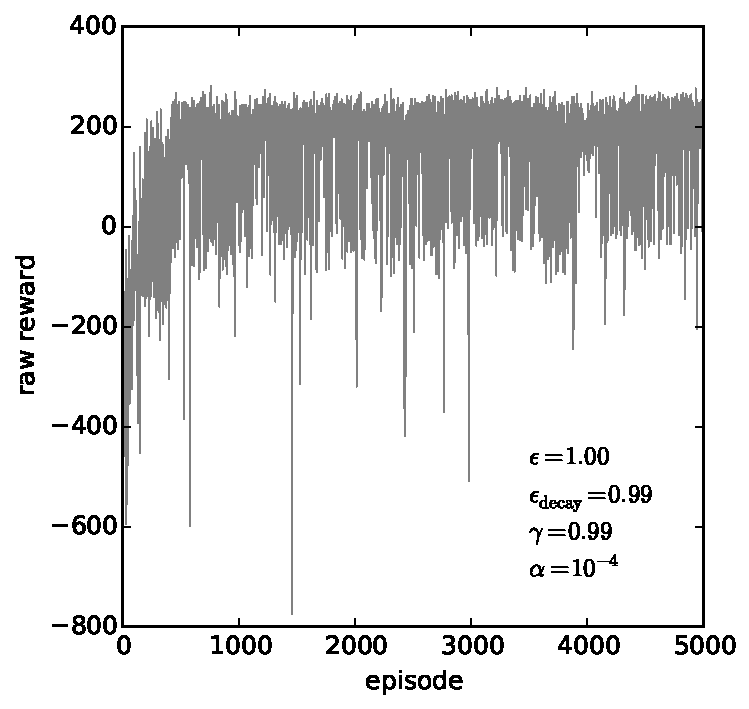
\includegraphics[width=0.45\textwidth]{./figures/fig1.pdf}
    \caption{Reward at each episode during agent training. The parameters used for training are shown. The agent receives a 100-episode average reward $>200$ at episode 1165 and is considered {\bf trained}. \label{fig:fig1}}
\end{figure}
\subsection{Behavior after training}
Fig.~\ref{fig:fig2} shows the smoothened version of Fig.~\ref{fig:fig1}. Here we've also shown the entire 20000 training episodes to highlight regions of {\bf overfitting}. The average reward is stable and between 150 and 200 for episodes between  1165 and $\sim$ 14000. After that we enter the regime of overfitting as seen from the rapid drop and downward trend in the average reward. Overfitting occurs when the weights in the network which whould be zero assume large nonzero values due to continued training. This is a well known phenomenon in neural net training which leads to a recommendation of {\bf early stopping}. We deliberately continued to overtrain to illustrate or point. In applications we'd recommend stopping at around 5000 episodes for this particular problem.
%%
\begin{figure}[tbp]
    \centering
    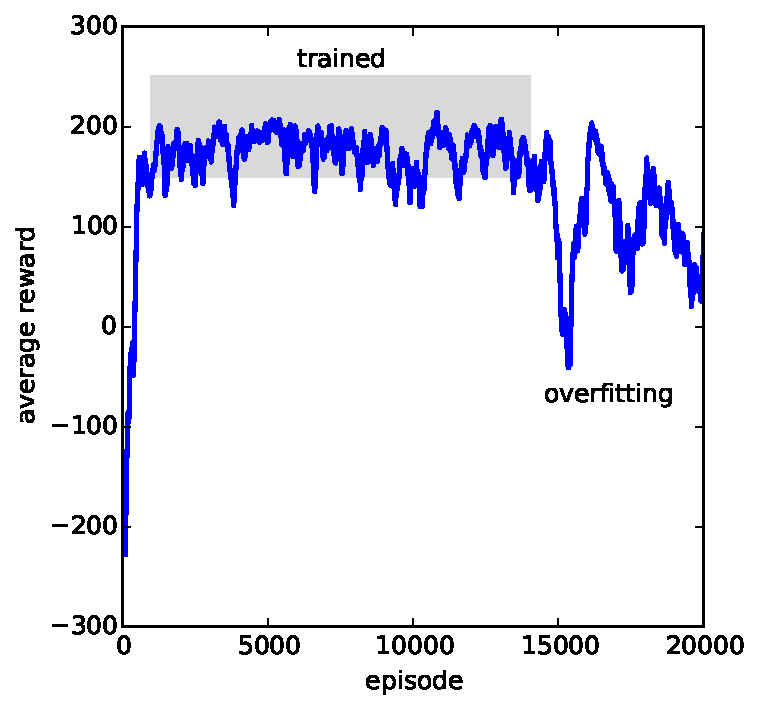
\includegraphics[width=0.45\textwidth]{./figures/fig2.pdf}
    \caption{(a) 100-episode average reward during entire training showing the regions of training, trained and overtraining/overfitting. (b) Demonstration of {\bf reproducibility} of training. Three agents trained using three different exploration strategies. The adaptation strategy used is depicted in the ineset of Fig.~\ref{fig:lr}(c).\label{fig:fig2}}
\end{figure}
%%
\section*{Summary}
Building the lunar lander control module taught us model-free learning with generalization. We evaluated linear, support vector, and neural net regressors as well as regression trees. Within our limited experiments, we found neural nets to provide the best out-of-the-box performance for lunar lander $Q$ function generalization. For neural nets we fixed two hidden layers but experimented with number of hidden nodes, number of training epochs, learning rate and batch size. We found a range of these parameters which provides {\bf reproducible} and {\bf stable} training for our agent. Finally our RL experiments with the discount rate and the exploration strategy demonstrated the considerable effect of the discount rate on the optimization of the agent.  With the learning in this exercise, we can build simple agents for other similar tasks including the walking robot, pong and mazes. 
\begin{thebibliography}{1}
\bibitem{dqn}
V.~Mnih et al., ``Playing Atari with Deep Reinforcement Learning,'' {\em arXiv:1312.5602 [cs.LG]} 2013.
\bibitem{suttonbarto}
Richard~S.~Sutton and Andrew~G.~Barto, ``Reinforcement Learning,'' {\em MIT Press}, 1998.
\end{thebibliography}

\end{document}


